\begin{figure}[htbp]
    \begin{center}
        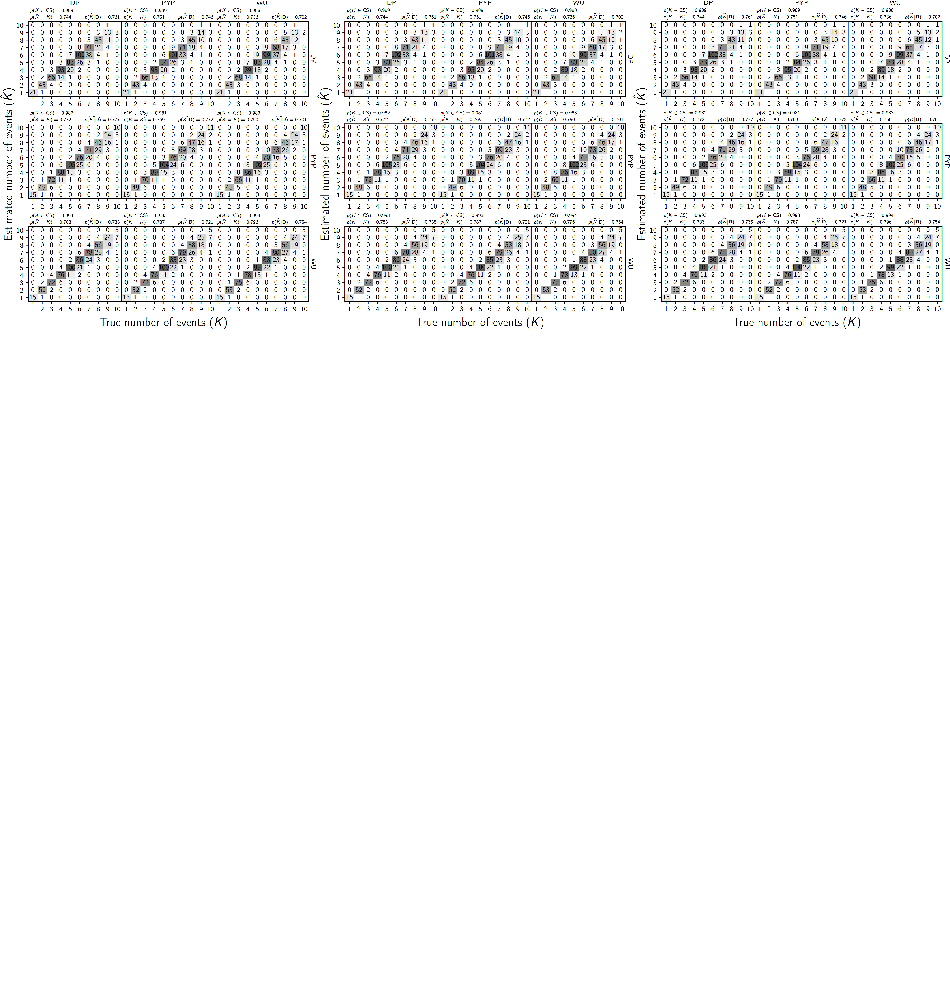
\includegraphics[width=\textwidth,height=\textheight,keepaspectratio]{../images/from-project-repo/infer-columns-by-data-rows-nevents-cropped-rasterized.pdf}
        \captionsetup{name=Figure S, labelformat=noSpace, listformat=sFigList}
        \caption{
        The models perform similarly in estimating the number of divergence
        events.
        Each plot shows the results for 720 \datasets
        simulated under the
        DP (top row),
        PYP (middle row),
        or
        WU (bottom row)
        and analyses using the
        DP (left column),
        PYP (middle column),
        or
        WU (right column).
        The number of \datasets that fall within each possible cell of true
        versus estimated numbers of events is shown, and cells with more
        \datasets are shaded darker.
        % The estimates are based on the number of events with the maximum
        % \textit{a posteriori} (MAP) probability.
        Above each plot is
        the proportion of \datasets for which the number of events with the largest
        posterior probability matched the true number of events---$p(\hat{\nevents}
        = \nevents)$,
        the median posterior probability of the correct number of events across all
        \datasets---$\widetilde{p(\nevents|\alldata)}$, and
        the proportion of \datasets for which the true number of events was
        included in the 95\% credible set---$p(\nevents \in
        \textrm{CS})$.
        We generated the plot using matplotlib Version 3.1.3
        \citep{matplotlib}.
        }
        \label{fig:neventsgrid}
    \end{center}
\end{figure}

\begin{figure}[htbp]
    \begin{center}
        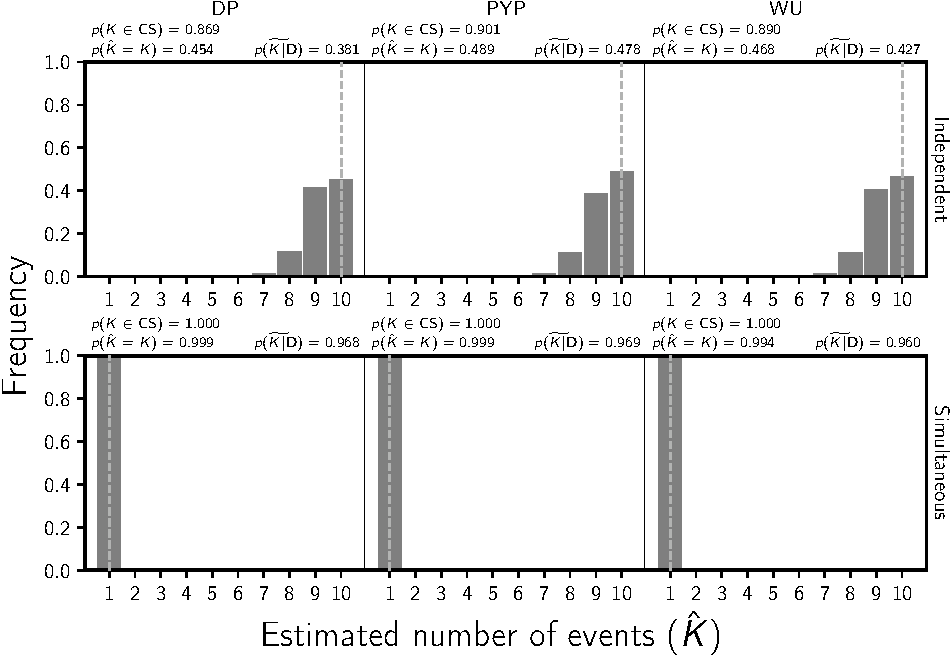
\includegraphics[width=\textwidth,height=\textheight,keepaspectratio]{../images/from-project-repo/infer-columns-by-fixed-rows-nevents-cropped.pdf}
        \captionsetup{name=Figure S, labelformat=noSpace, listformat=sFigList}
        \caption{
        The PYP (middle column) model performs better than the DP (left column)
        and WU (right column) models when analyzing simulated \datasets for
        which all 10 population pairs diverged independently (top row).
        All three models almost always correctly infer a single shared
        divergence event with high confidence when analyzing simulated
        \datasets for which that is true (bottom row).
        Each plot shows the results for 720 \datasets.
        Above each plot is
        the proportion of \datasets for which the number of events with the largest
        posterior probability matched the true number of events---$p(\hat{\nevents}
        = \nevents)$,
        the median posterior probability of the correct number of events across all
        \datasets---$\widetilde{p(\nevents|\alldata)}$, and
        the proportion of \datasets for which the true number of events was
        included in the 95\% credible set---$p(\nevents \in
        \textrm{CS})$.
        We generated the plot using matplotlib Version 3.1.3
        \citep{matplotlib}.
        }
        \label{fig:neventsfixedcomparison}
    \end{center}
\end{figure}
